\scanpage{77}
% archive foliation: 76
\diagram{\begin{tikzcd}[ampersand replacement=\&,column sep=small]
\& R\arrow[dl,"p"']\arrow[d,bend right=15,"q'"']\arrow[d,bend left=15,"q''"]\arrow[dr,"r"]\&\\
S\&A\&F
\end{tikzcd}}
\diagram{\begin{tikzcd}[ampersand replacement=\&,column sep=large]
\& R^\circ=R\arrow[dl,"p^\circ=p"']\arrow[d,bend right=15,"q'{}^\circ=q''"']\arrow[d,bend left=15,"{q''{}^\circ=\deleted{\unsure{q'}}\inserted{q'\circ\sigma_2}}"]\arrow[dr,"{\unsure{q|r}^\circ=\unsure{q|r}\circ\sigma_2}"]\&\\
S\&A\&F
\end{tikzcd}}

\figure{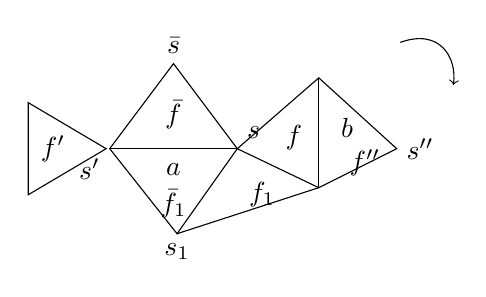
\begin{tikzpicture}[scale=.9]
\draw (-3.1,-.65)--(-3.1,.65)--(-2,0)--cycle;
\draw (-1.95,0)--(-1.05,1.2)--(-.15,0)--(-1,-1.2)--cycle;
\draw (-1.95,0)--(-.15,0);
\draw (-.15,0)--(1,1)--(2.1,0)--(1,-.55)--cycle;
\draw (1,1)--(1,-.55);
\draw (-1,-1.2)--(1,-.55);
\node at (-2.75,0) {$f'$};
\node[below left] at (-1.95,0) {$s'$};
\node[above right] at (-.15,0) {$s$};
\node[above] at (-1.05,1.2) {$\bar s$};
\node at (-1.05,.48) {$\bar f$};
\node at (-1.05,-.3) {$a$};
\node at (-1.05,-.78) {$\bar f_1$};
\node[below] at (-1,-1.2) {$s_1$};
\node at (.65,.15) {$f$};
\node at (1.4,.3) {$b$};
\node at (1.65,-.2) {$f''$};
\node[right] at (2.1,0) {$s''$};
\node at (.2,-.65) {$\unsure{f_1}$};
\draw[->] (2.15,1.5) .. controls (2.7,1.7) and (2.95,1.3) .. (2.9,.9);
\end{tikzpicture}}
\[
\begin{aligned}
p(s,f)&=s & \sigma_0(s,f)&=(s',f')\\
r(s,f)&=f & \sigma_2(s,f)&=(s'',f'')\\
q'(s,f)&=a\\
q''(s,f)&=b
\end{aligned}
\]
\[
\sigma_0\sigma_2(s,f)=\sigma_2\sigma_0(s,f)=(s'',f'')
\]
\[
E=(R,q')\times_A(R,q'')=
\left\{\overbrace{((s,f),(\bar s,\bar f))}^{\text{\unsure{remplacer}}\ (s,a,\bar f)}
\mid q'(s,f)=q''(\bar s,\bar f)\right.
\]
\inserted{$\unsure{''}$}
\diagram{\begin{tikzcd}[ampersand replacement=\&,column sep=small]
\&E\arrow[dl,"\pi_{01}"']\arrow[d,"\pi_{02}"]\arrow[dr,"\pi_{12}"]\&\\
R\&R\&R
\end{tikzcd}}
\[
\begin{aligned}
\pi_{01}^+(s,f,\bar s,\bar f)&=(s,f)\\
\pi_{12}^+(s,f,\bar s,\bar f)&=(\bar s,\bar f)\\
\pi_{02}^+(s,f,\bar s,\bar f)&=(s,\bar f)
\end{aligned}
\]
\[
E^+=\left\{(s,f,\bar s,\bar f)\in E\mid (s,a,\bar f)\ \unsure{direct}\right.
\]
\inserted{$a=q'(s,f)=q''(\bar s,\bar f)$}
\[
\left\{\begin{aligned}
\sigma_0(s,f,\bar s,\bar f)&=(s,f_{\unsure{2|1}}\deleted{\unsure{)}},\bar s,\bar f)\\
\sigma_1(s,\unsure{f|\bar f},\bar s,\bar f)&=(s,f_1,\unsure{\underline{s'}|\bar s'},\unsure{\underline{\bar f}|\bar{\bar f}})\\
\sigma_2(s,f,\bar s,\bar f)&=(s,f,\bar s_1,f_1)
\end{aligned}\right.
\]
\diagram{\begin{tikzcd}[ampersand replacement=\&,column sep=large]
\&E^+\arrow[dl,"\pi_{01}^+"']\arrow[d,"\pi_{02}^+"]\arrow[dr,"\pi_{12}^+"]\&\\
R\&R\&R\\
\&E^-\arrow[ul,"\pi_{01}^-" ]\arrow[u,"\pi_{02}^-"']\arrow[ur,"\pi_{12}^-"']\&
\end{tikzcd}}
\diagram{\begin{tikzcd}[ampersand replacement=\&]E^+\\[5em]E^-\end{tikzcd}}
